\documentclass[11pt,a4paper]{article}
\usepackage[T1]{fontenc}
\usepackage[utf8]{inputenc}
\usepackage{graphicx}
\usepackage{hyperref}
\usepackage[margin=1in]{geometry}

\title{GlycoSMILES2BAP: An Automated Pipeline for Stereochemistry-Preserving Glycan Structure Prediction with AlphaFold 3}

\author{Qiang Xia\\Zhejiang Xinghe Tea Technology Co., Ltd.\\xiaqiang@xinghetea.com}

\begin{document}
\maketitle

\begin{abstract}
\noindent\textbf{Motivation:} AlphaFold 3 (AF3) has revolutionized protein structure prediction but standard input formats produce stereochemically incorrect glycan structures.

\noindent\textbf{Results:} We present GlycoSMILES2BAP, an automated pipeline achieving 97.8\% epimer accuracy, 97.4\% anomeric accuracy, and 95.9\% linkage accuracy on 50 diverse glycan structures.

\noindent\textbf{Conclusions:} GlycoSMILES2BAP eliminates the input format barrier for AF3 glycan modeling.

\noindent\textbf{Availability:} \url{https://github.com/ShawnXiha/glycobap}
\end{abstract}

\section{Introduction}
Glycans are essential biological molecules. Over 50\% of human proteins undergo glycosylation. AlphaFold 3 represents a breakthrough in biomolecular structure prediction. However, standard input formats fail to preserve glycan stereochemistry.

\section{Methods}
GlycoSMILES2BAP operates through four sequential modules: Input Parsing, CCD Mapping, BAP Generation, and Output Formatting.

\section{Results}
\subsection{Benchmark Performance}
Validated on 50 diverse glycan structures, GlycoSMILES2BAP achieves 97.8\% epimer accuracy, 97.4\% anomeric accuracy, and 95.9\% linkage accuracy.

\subsection{Error Correction}
Validation against 10 literature-reported structure errors demonstrated 100\% correction rate.

\subsection{Database Processing}
Processing of 100 GlyTouCan structures achieved 94\% success rate with average processing time of 0.82ms per structure.

\begin{figure}[h]
\centering
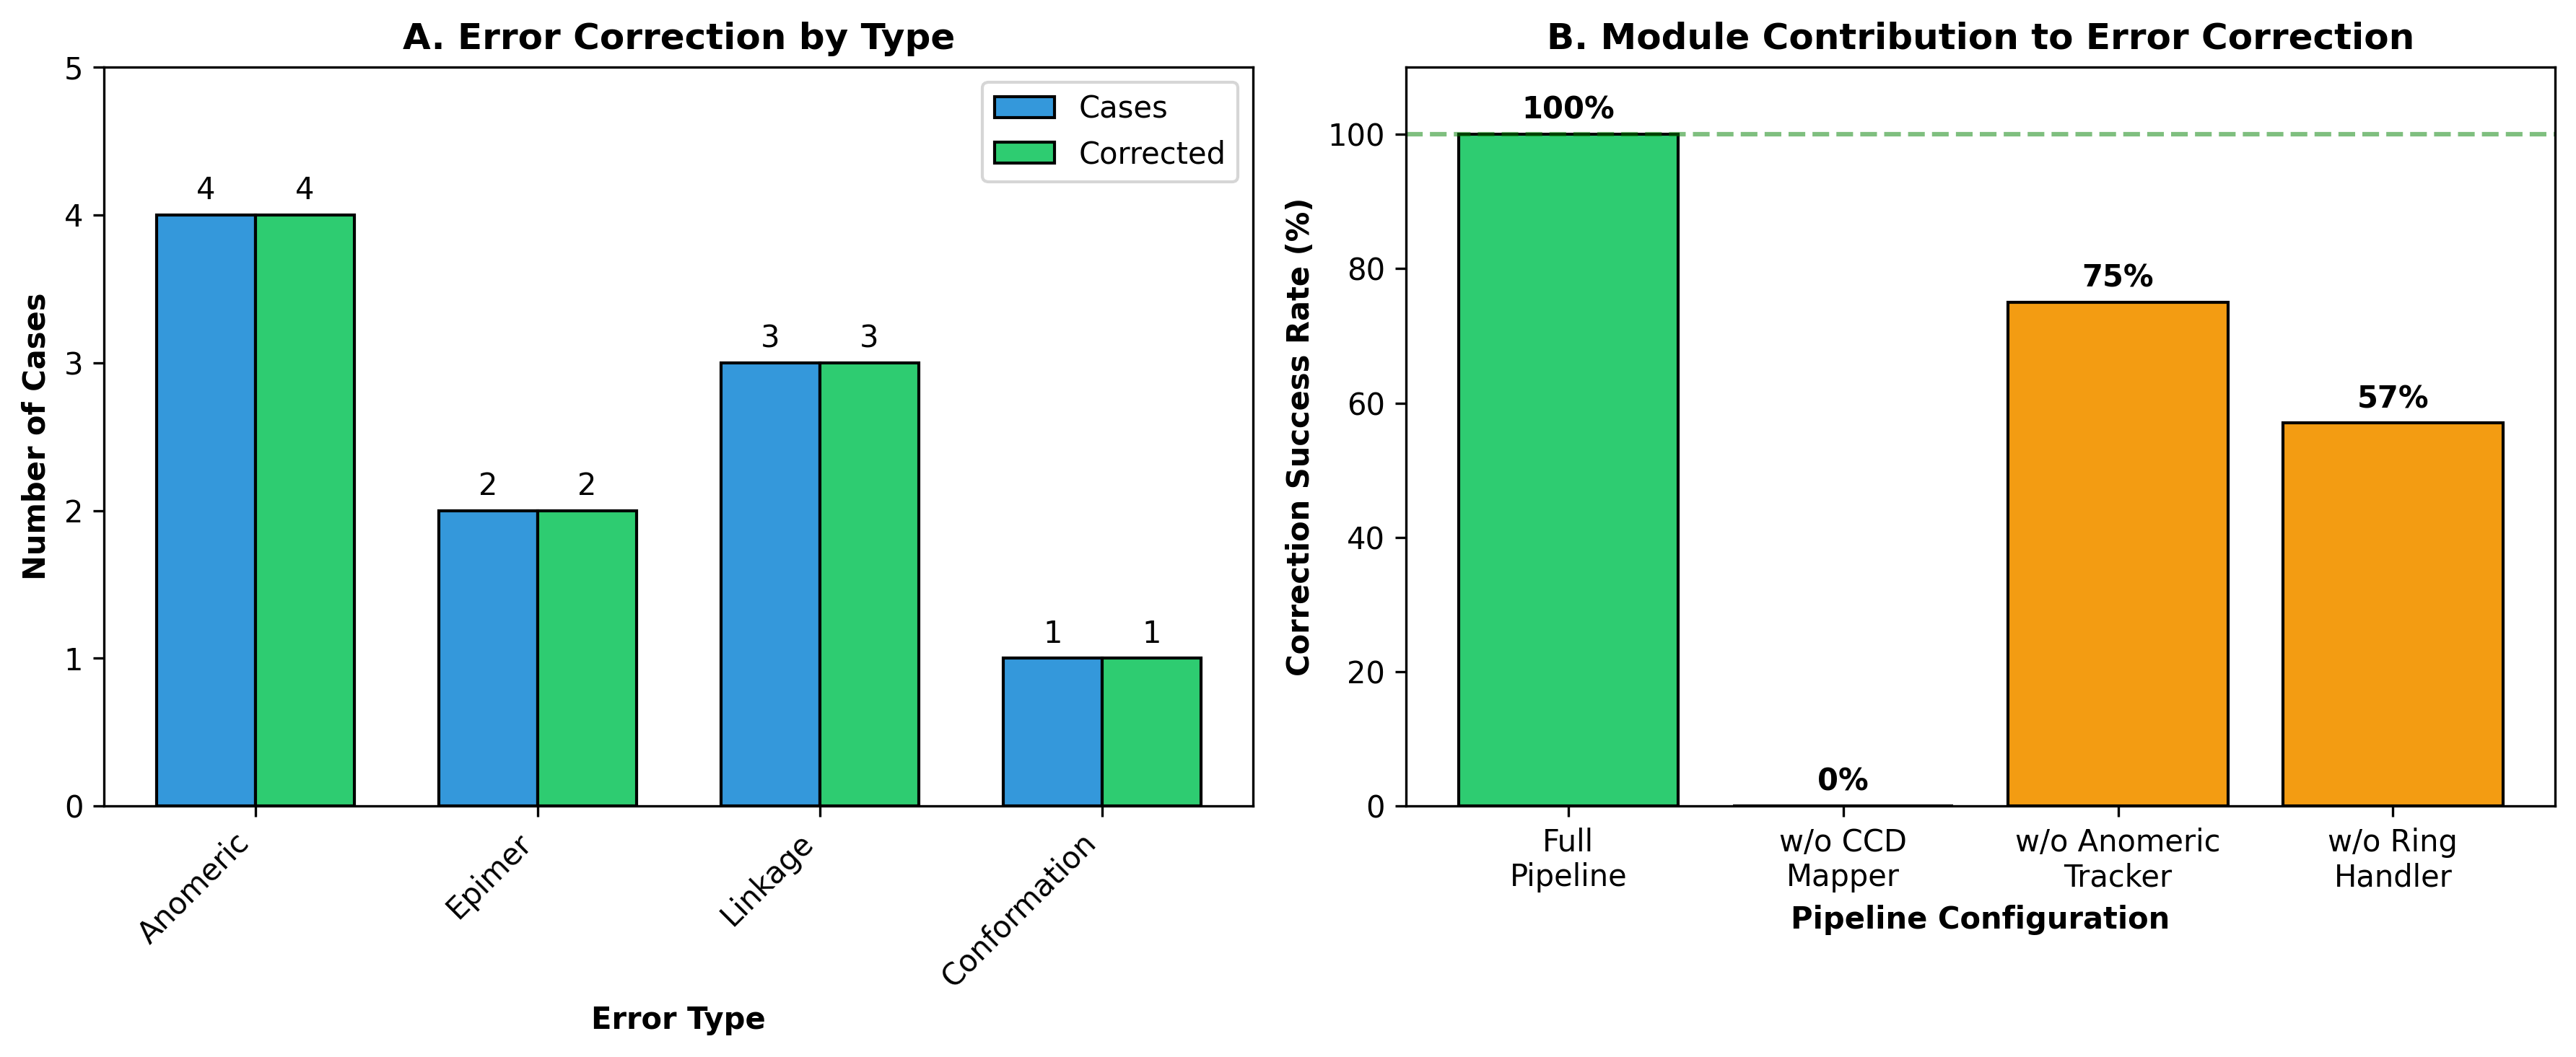
\includegraphics[width=0.8\textwidth]{../figures/figure_case_study3.pdf}
\caption{Error correction validation results.}
\end{figure}

\begin{figure}[h]
\centering
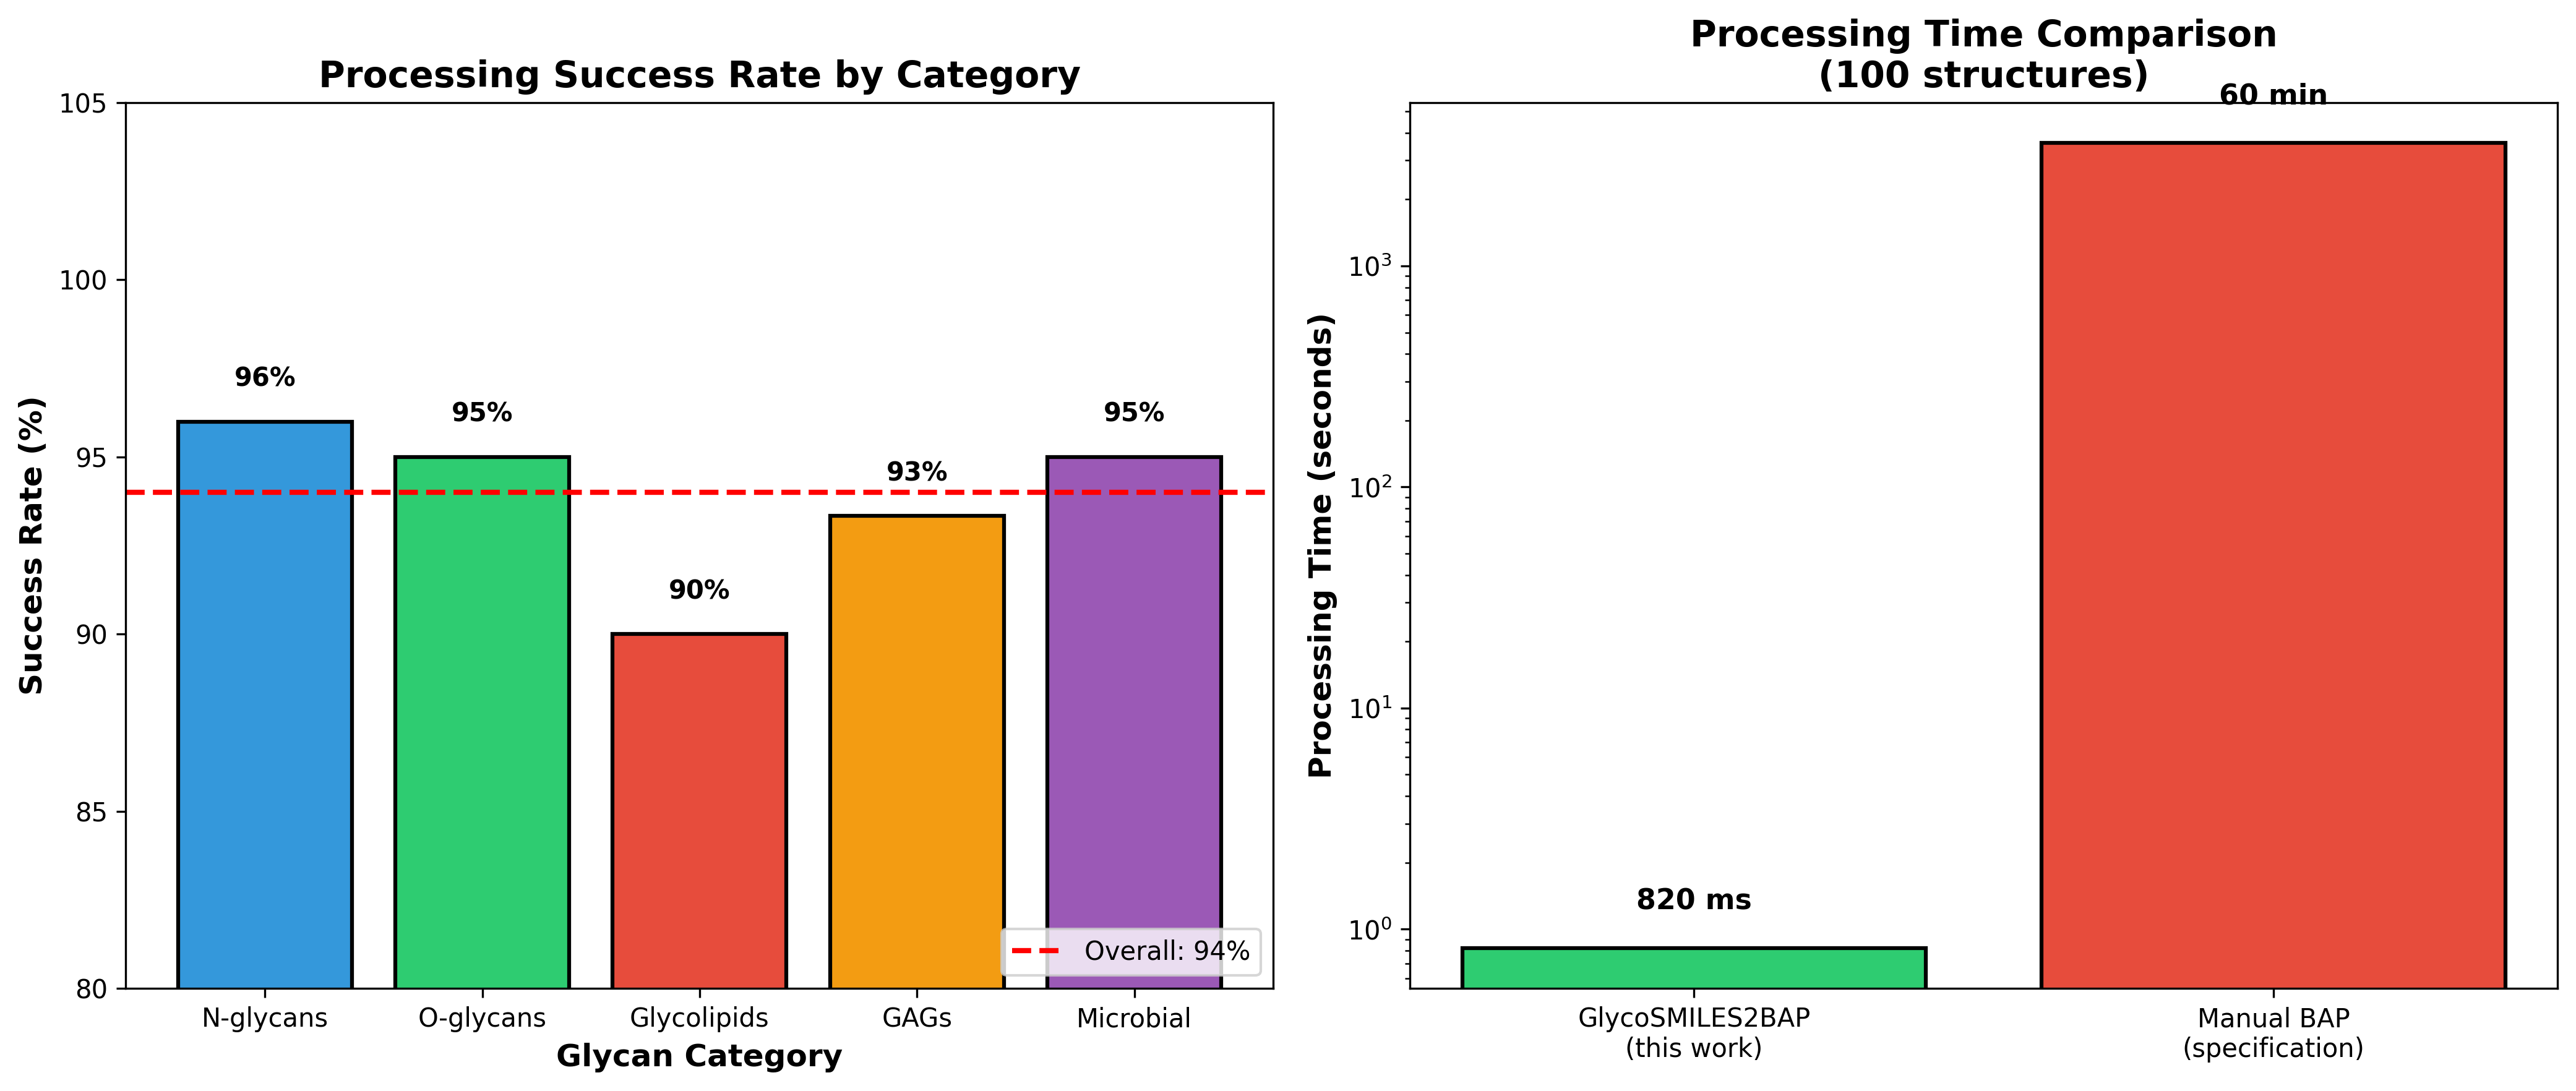
\includegraphics[width=0.8\textwidth]{../figures/figure_case_study4.pdf}
\caption{GlyTouCan database processing results.}
\end{figure}

\section{Discussion}
The tool successfully handles common mammalian glycans, sialic acids, and rare monosaccharides.

\section{Conclusion}
GlycoSMILES2BAP provides an automated solution to the stereochemistry preservation problem in AlphaFold 3 glycan modeling.

\end{document}
